\documentclass[10pt]{beamer}

\usepackage{amssymb, amsmath, fleqn}
\usepackage{graphicx, graphics, tikz}
\usepackage{color}
\usepackage{tabu}

\newtheorem{thm}{Theorem}
\newtheorem{acknowledgement}[thm]{Acknowledgement}
\newtheorem{algorithm}[thm]{Algorithm}
\newtheorem{axiom}[thm]{Axiom}
\newtheorem{case}[thm]{Case}
\newtheorem{claim}[thm]{Claim}
\newtheorem{proposition}[thm]{Proposition}
\newtheorem{rmrk}[thm]{Remark}
\newtheorem{summary}[thm]{Summary}

\let\oldsqrt\sqrt
\def\sqrt{\mathpalette\DHLhksqrt}
\def\DHLhksqrt#1#2{%
\setbox0=\hbox{$#1\oldsqrt{#2\,}$}\dimen0=\ht0
\advance\dimen0-0.2\ht0
\setbox2=\hbox{\vrule height\ht0 depth -\dimen0}%
{\box0\lower0.4pt\box2}}

\mode<presentation> {
    \usetheme[headheight=2.5ex]{boxes}
    \addheadbox{palette secondary}{\hspace*{4ex}\insertsection} %section on top
    \addheadbox{palette secondary}{\insertsubsection} %subsection on top (same color as section, so no split effects)
    \setbeamertemplate{footline}{\insertnavigation{\paperwidth}} %navigation (miniframe) on the bottom
    \setbeamertemplate{navigation symbols}{} %gets rid of navigation symbols
    \setbeamertemplate{caption}[numbered]
    \setbeamertemplate{blocks}[rounded][shadow=true]
    \setcounter{tocdepth}{2}

    \definecolor{VTMaroon}{RGB}{0,0,50}
    \definecolor{VTOrange}{RGB}{0,0,70}

    \setbeamercolor*{normal text}{fg=black,bg=white}
    \setbeamercolor*{alerted text}{fg=red}
    \setbeamercolor*{example text}{fg=black}
    \setbeamercolor*{structure}{fg=VTMaroon, bg=white}

    \setbeamerfont{alerted text}{series=\bfseries}

    \setbeamercolor*{palette primary}{fg=white,bg=VTMaroon}
    \setbeamercolor*{palette secondary}{fg=white,bg=VTOrange}
    \setbeamercolor*{palette tertiary}{fg=VTOrange,bg=VTMaroon}
    \setbeamercolor*{palette quaternary}{fg=white,bg=black}

    \setbeamercolor{titlelike}{fg=white, bg=VTMaroon}
    \setbeamercolor{frametitle}{fg=white, bg=VTMaroon}
    \setbeamercolor{frametitle right}{fg=white, bg=VTMaroon}

    \setbeamercolor{sidebar}{bg=VTOrange}

    \setbeamercolor*{palette sidebar primary}{fg=black}
    \setbeamercolor*{palette sidebar secondary}{fg=black}
    \setbeamercolor*{palette sidebar tertiary}{fg=black}
    \setbeamercolor*{palette sidebar quaternary}{fg=black}

    \setbeamercolor*{item projected}{fg=black,bg=black!20}

    \setbeamercolor{block title}{fg=white,bg=VTOrange}
    \setbeamercolor{block title alerted}{use=alerted text,fg=white,bg=alerted text.fg!75!black}
    \setbeamercolor{block title example}{use=example text,fg=white,bg=example text.fg!75!black}

    \setbeamercolor{block body}{parent=normal text,use=block title,bg=block title.bg!15!bg}
    \setbeamercolor{block body alerted}{parent=normal text,use=block title alerted,bg=block title alerted.bg!15!bg}
    \setbeamercolor{block body example}{parent=normal text,use=block title example,bg=block title example.bg!15!bg}

    \setbeamercolor*{separation line}{}
    \setbeamercolor*{fine separation line}{}
}

\newcounter{llst}
\newenvironment{abet}{\begin{list}{\rm (\alph{llst})}{\usecounter{llst}
\setlength{\itemindent}{0em} \setlength{\leftmargin}{3em}
\setlength{\labelwidth}{2em} \setlength{\labelsep}{1em}}}{\end{list}}
\newenvironment{numm}{\begin{list}{\rm (\roman{llst})}{\usecounter{llst}
\setlength{\itemindent}{0em} \setlength{\leftmargin}{3.5em}
\setlength{\labelwidth}{2.5em} \setlength{\labelsep}{1em}}}{\end{list}}

\title[EntrepreneurshipSSE]{\textcolor{yellow}{Entrepreneurship and Wealth-Generation in Socially Structured Economies}}
\subtitle{An Overview}
\author[Sims]{Owen~Sims}
\institute[QUB]{Center for Data Science and Scalable Computing\\ Queen's University Belfast}
\date[APR 2016]{QMS Annual Progress Review, September 2016}

\begin{document}

\begin{frame}
\titlepage
\end{frame}

\section{Overview of dissertation}

\begin{frame}
\frametitle{Table of contents}
\tableofcontents
\end{frame}

\begin{frame}
\frametitle{Table of contents}
\tableofcontents[currentsection]
\end{frame}

\subsection{Introduction}

\begin{frame} \frametitle{Introduction}
\begin{quotation}
``[T]here is hardly any part of economics that would not be advanced by a further analysis of specialisation.''
\end{quotation}
\begin{flushright}
---Hendrik Houthakker (1956, p. 182)
\end{flushright}
\begin{quotation}
``Static models provided by traditional equilibrium theory do nothing to explain the most central concept in economic development: the entrepreneur.''
\end{quotation}
\begin{flushright}
---Coase and Wang  (2012, p. 1)
\end{flushright}
\begin{itemize}
\medskip
\item We present theoretical and empirical considerations in the field of entrepreneurship by investigating the interaction between \emph{institutions}, \emph{networks} and the \emph{social division of labour}.
\medskip
\end{itemize}
\end{frame}


\begin{frame} \frametitle{Fundamental idea}
\begin{itemize}
\item The act of entrepreneurship is expressed through a crucial development of the social division of labour. 
\medskip
\item This is reflected in a major modification of institutional environments and networked interaction infrastructures.
\medskip
\item We investigate the conjecture that entrepreneurial activities by individuals and coalitions lead to new specialisations, \emph{socio-economic roles} and, as a consequence, unique positions in the economy.
\medskip
\begin{itemize}
\item Entrepreneurial positions are \emph{uncontested} such that they can lead to exploitation.
\medskip
\item However, they are also wealth-generating positions, facilitating deeper divisions of labour and the connection of communities that would otherwise be disconnected.
\end{itemize}
\end{itemize}
\end{frame}

\subsection{Dissertation structure}

\begin{frame} \frametitle{Dissertation structure}
\begin{itemize}
\item The analysis of entrepreneurship within a network-institutional---or \emph{relational}---perspective is partitioned into three consecutive Parts:
\medskip
\begin{itemize}
\item[\textbf{Part I.}] Develops a theory of economic interaction, wealth-generation and entrepreneurship within a \emph{socially structured economy}.
\medskip
\item[\textbf{Part II.}] Investigates entrepreneurial activity and positional power in an economy consisting of a horizontal division of labour.
\medskip
\item[\textbf{Part III.}] Investigates entrepreneurial activity and positional power in with more complex interaction structures and a vertical division of labour.
\end{itemize}
\medskip
\item Throughout we complement theory with empirical examples; this includes the analysis of elite Florentine families and the directorate network of New York City during the early Twentieth Century.
\end{itemize}
\end{frame}


\begin{frame} \frametitle{Current status}
\begin{itemize}
\item Submitted: \textbf{Thursday 8th September 2016}.
\medskip
\item Viva date has been confirmed with internal and external examiners and has been booked for \textbf{Thursday 24th November 2016}.
\medskip
\item Dissertation with associated files, code, data and presentations (including this) can be forked from the dedicated Github repository: \href{https://github.com/OwenSims/EntrepreneurshipSSE}{https://github.com/OwenSims/EntrepreneurshipSSE}.
\medskip
\item Two chapters---\emph{Middlemen as entrepreneurs} and \emph{The formation of extractive structures in networks}---have been transformed into papers and were well-received in conferences.
\medskip
\item Tools developed within the monograph to analyse power in topological environments have been integrated into open source statistical packages in R (\emph{networkR}) and Python (\emph{iGraph}).
\end{itemize}
\end{frame}

\section{Developing a Theory of Entrepreneurship}

\begin{frame}
\frametitle{Table of contents}
\tableofcontents[currentsection]
\end{frame}

\subsection{Overview of Part I}

\begin{frame} \frametitle{Part I overview}
\begin{itemize}
\item Part I develops, from an axiomatic basis, a set of fundamental notions that inform the relational perspective. From this we define the entrepreneur and entrepreneurial activity.
\medskip
\item Part I results in:
\begin{itemize}
\medskip
\item[1.] Formal definition of \emph{socially structured economies} given a relational perspective of social and economic activity.
\medskip
\item[2.] Development of consumer-producers, socio-economic roles and the social division of labour.
\medskip
\item[3.] Clarity regarding the definition and impact of entrepreneurship and the entrepreneurial function within this framework.
\end{itemize}
\medskip
\item This is expressed over three chapters.
\end{itemize}
\end{frame}

\subsection{Toward a relational perspective}

\begin{frame} \frametitle{Chapter 1: Toward a relational perspective}
\begin{itemize}
\item This chapter provides and debates the fundamental modelling axioms and hypotheses required to develop the relational perspective.
\begin{itemize}
\medskip
\item[\textbf{Axiom I.}] \textbf{Bounded rationality:} Limited cognitive abilities to compute the consequences of their own and others actions. This results into fundamental perceived uncertainty in the economy.
\medskip
\item[\textbf{Axiom II.}] \textbf{Harmonisation of production and consumption:} Economic agents are bearers of consumptive needs as well as productive abilities.
\end{itemize}
\medskip
\item The following notions are derived from these axioms: (1) Economic agents as consumer-producers; (2) Socio-economic roles and specialisations; (3) Embeddedness, governance systems, and institutions; and (4) Interaction infrastructures as networks.
\end{itemize}
\end{frame}


\begin{frame}
\begin{itemize}
\item Economic agents are assumed to be identical and possess both consumption and production functions consisting of increasing returns to specialisation over the set of produceable economic goods.
\end{itemize}
\begin{figure}[h]
\centering
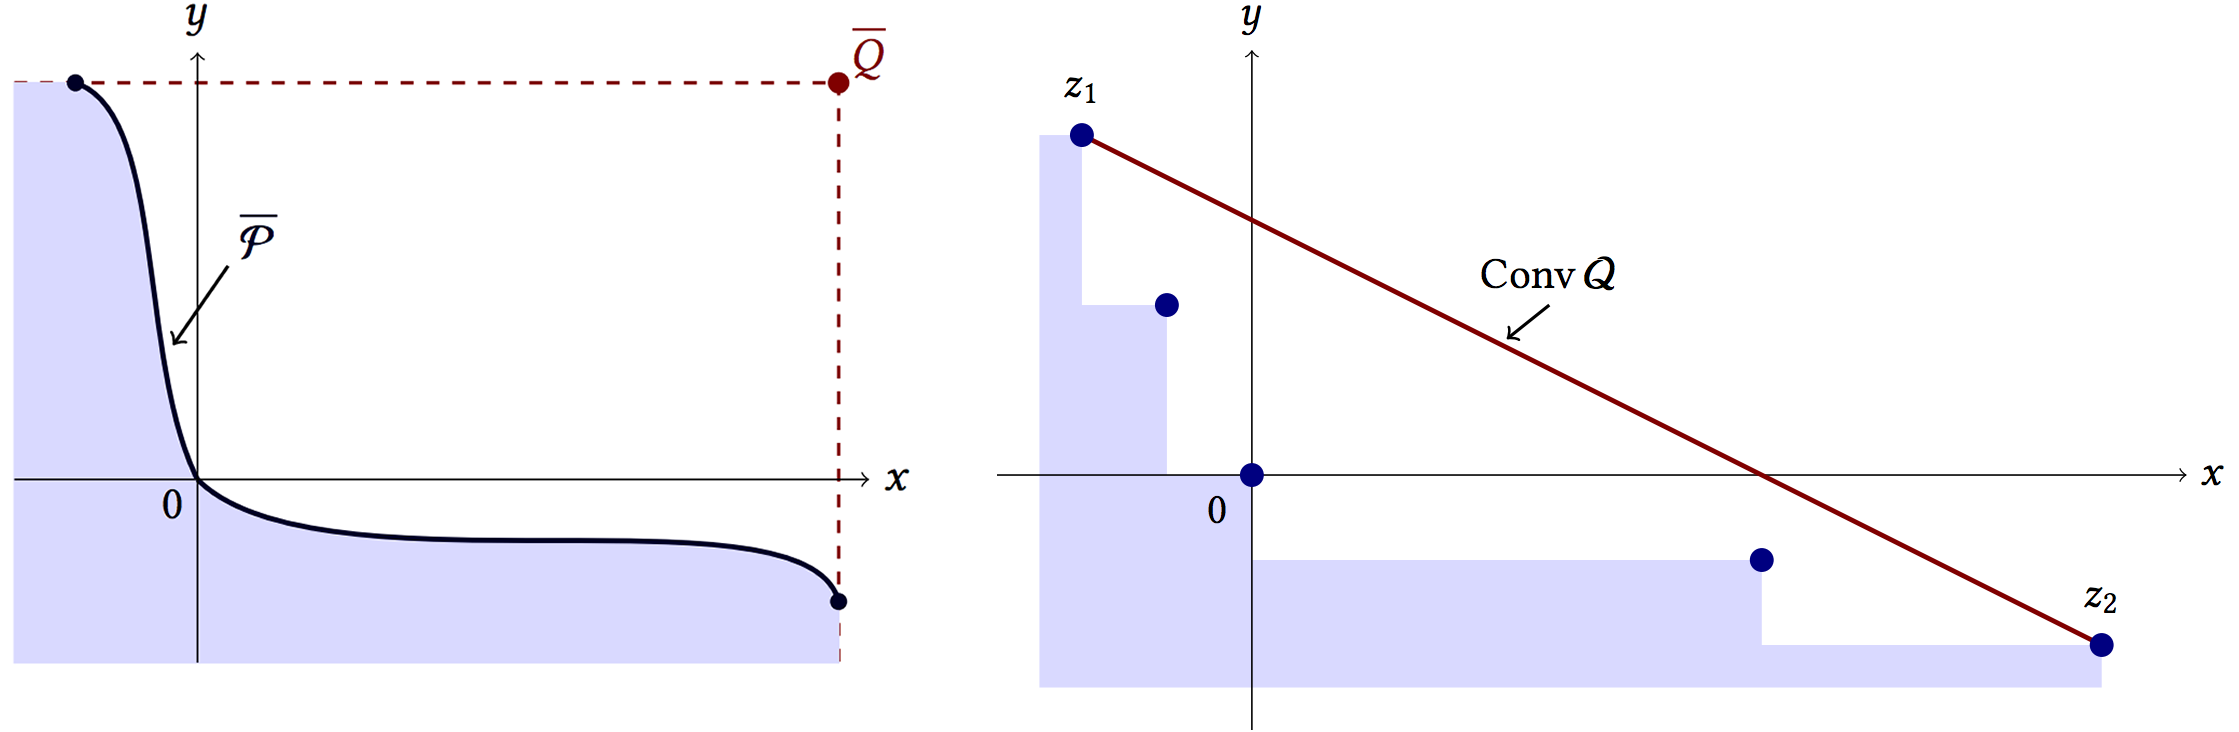
\includegraphics[scale=0.135]{../Images/IRS.png}
\end{figure}
\begin{itemize}
\item The assumption of strict IRS leads to the theorem that, given a population of $> 1$ economic agents and no interaction inefficienies, each agent always has an incentive to specialise.
\end{itemize}
\end{frame}


\begin{frame}
\begin{itemize}
\item To engage in functional wealth-generating interaction each agent adopts a specialisation and with it a socio-economic role.
\medskip
\item A socio-economic role expresses an agents \emph{embeddedness} in a well-defined governance system.
\medskip
\begin{figure}[h]
\begin{center}
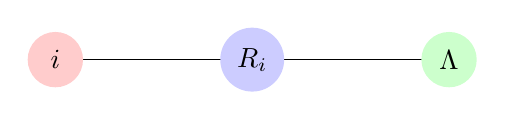
\begin{tikzpicture}[scale=0.25]
\draw (0,0) -- (20,0);
\draw (20,0) node[minimum size=2em,circle,fill=green!20] {$\Lambda$};
\draw (0,0) node[minimum size=2em,circle,fill=red!20] {$i$};
\draw (10,0) node[minimum size=2em,circle,fill=blue!20] {$R_{i}$};
\end{tikzpicture}
\end{center}
\end{figure}
\medskip
\item A socio-economic role is a reflection of the governance system ($\Lambda$) that an agent exists within. 
\begin{itemize}
\medskip
\item Includes behavioural rules, cultural norms, media that are associated with specialisations.
\end{itemize}
\medskip
\item Economic agents adopt a socio-economic role through either \emph{adaptive specialisation} or \emph{objective specialisation}.
\end{itemize}
\end{frame}


\begin{frame} %\frametitle{}
\begin{figure}[h]
\begin{center}
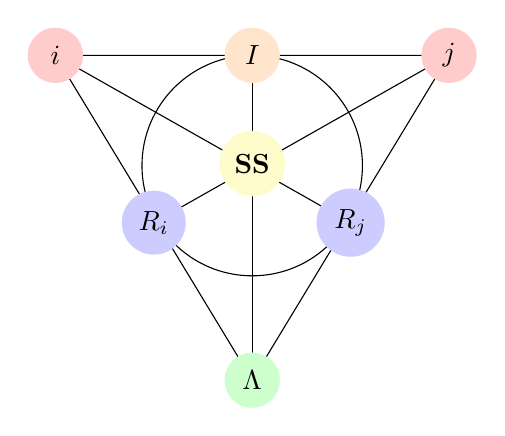
\begin{tikzpicture}[scale=0.25]
\draw (0,17) -- (10,0.5) -- (20,17) -- (0,17);
\draw (10,0.5) -- (10,17);
\draw (0,17) -- (15,8.5);
\draw (20,17) -- (5,8.5);
\draw (10,11.4) circle (5.6cm) ;
\draw (10,0.5) node[minimum size=2em,circle,fill=green!20] {$\Lambda$};
\draw (0,17) node[minimum size=2em,circle,fill=red!20] {$i$};
\draw (20,17) node[minimum size=2em,circle,fill=red!20] {$j$};
\draw (10,17) node[minimum size=2em,circle,fill=orange!20] {$I$};
\draw (5,8.5) node[minimum size=2em,circle,fill=blue!20] {$R_i$};
\draw (15,8.5) node[minimum size=2em,circle,fill=blue!20] {$R_j$};
\draw (10,11.5) node[minimum size=2em,circle,fill=yellow!20] {\textbf{SS}};
\end{tikzpicture}
\end{center}
\end{figure}
\begin{itemize}
\item Due to the problem of the Core economic agents are considered as centrifugal forces and the governance system as a centripetal force.
\medskip
\item The fundamental problem of the Core needs to be resolved through the use of institutional mechanisms.
\end{itemize}
\end{frame}


\begin{frame} %\frametitle{}
\begin{itemize}
\item The formation of economic relationships leads to a global social structure termed as an \textbf{interaction infrastructure}.
\medskip
\item An interaction infrastructure refers to a tuple consisting of:
\begin{itemize}
\medskip
\item[1.] A population of consumer-producers; and
\medskip
\item[2.] A set of functional bilateral economic interactions and relationships formed between the population of consumer-producers.
\end{itemize}
\medskip
\item Interaction infrastructures are represented as \emph{networks}.
\medskip
\item Leads to the modelling Lemma regarding the positional attributes of economic agents: 
\begin{itemize}
\medskip
\item Economic agents have a relational position within an interaction infrastructure. These positional attributes are derived from the economic interactions they form with others.
\end{itemize}
\end{itemize}
\end{frame}

\subsection{Growth and development of the socio-economic space}

\begin{frame} \frametitle{Chapter 2: Growth \& development of the socio-economic space}
\begin{itemize}
\item All economic relationships and interactions are socially embedded and exist within some well-defined \emph{space}. 
\begin{itemize}
\medskip
\item We term this interaction space as a \textbf{socio-economic space}.
\medskip
\item Refers to a given set of economic agents engaged in a well-described collection of general economic interactions that operate under a well-defined collection of media and institutions.
\medskip
\item As such, the socio-economic space contains economic agents, interaction infrastructures, and a governance system guiding the formation of these relationships.
\end{itemize}
\medskip
\item This Chapter provides an overview of the socio-economic space and, with it, an analysis and simulation of its growth and development through adaptive specialisation.
\end{itemize}
\end{frame}


\begin{frame}
\begin{figure}[h]
\centering
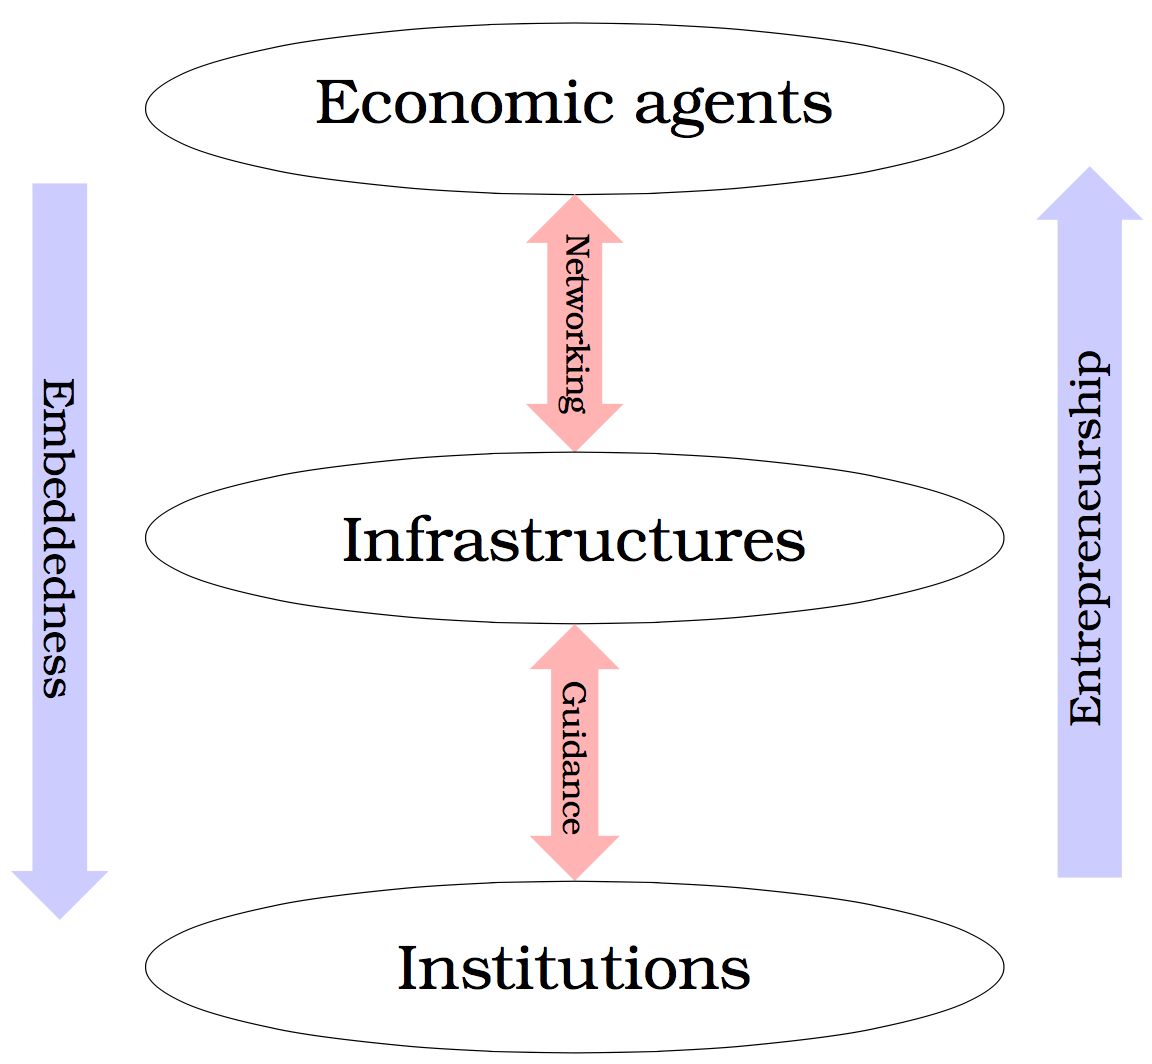
\includegraphics[scale=0.135]{../Images/structure-space.png}
\end{figure}
\begin{itemize}
\item There exists a two-way relationship between the population of economic agents, their relational position within the economy and the set of institutions in the governance system.
\end{itemize}
\end{frame}


\begin{frame}
\begin{itemize}
\item The socio-economic space is defined in a formal manner as a mathematical concept.
\medskip
\item A socio-economic space can be represented by a pair $(N, \mathcal{G})$ where $N = \{1, \ldots, n\}$ is a given set of economic agents and
\begin{equation*}
\mathcal{G} \subset \mathcal{S}(N) \cup \mathcal{H}(N)
\end{equation*}
is a given collection of \textbf{general economic interactions} on $N$, where
\begin{equation*}
\mathcal{S}(N) = \{ S ~ \mid ~ S \subset N \mbox{ and } S \neq \varnothing \}
\end{equation*}
is the family of non-empty coalitions in the population $N$, representing \textbf{lateral} economic interactions on $N$, and
\begin{equation*}
\mathcal{H}(N) = \bigcup_{k = 2}^{\infty} N^{k}
\end{equation*}
is the class of all finite ordered sequences of economic agents, representing \textbf{hierarchical} economic interactions in $N$.
\end{itemize}
\end{frame}


\begin{frame}
\begin{itemize}
\item Whilst discussing the evolution of the socio-economic space we distinguish the notions of growth and development.
\begin{itemize}
\medskip
\item \textbf{Growth:} Refers to a change in some fundamental or pre-existing parameters that define the socio-economic space such that the aggregate utility of all economic agents increases.
\medskip
\item \textbf{Development:} Refers to a productive change in the elements of the governance system and its derived structure such that the new institutional mechanisms, for example, produces an increase in aggregate utility.
\end{itemize}
\medskip
\item At this point we make the connection between \emph{the development of the socio-economic space and productive entrepreneurial activity} under the relational perspective.
\medskip
\item Further, we make a note that \textbf{decline} and \textbf{regression} are polar notions to growth and development.
\end{itemize}
\end{frame}


\begin{frame}
\begin{itemize}
\item The growth of the socio-economic space is simulated through the process of adaptive specialisation.
\medskip
\item A number of simulations are provided (written in Matlab). Each simulation differs in a number of factors:
\begin{itemize}
\medskip
\item[1.] The relative production technologies/abilities of the economic agents in the outputs considered; and
\medskip
\item[2.] The exchange mechanisms considered that characterise the socio-economic space.
\end{itemize}
\medskip
\item Simulations define two environments within which economic agents operate. These environments are informed through different exchange mechanisms:
\begin{itemize}
\medskip
\item[1.] Egalitarian exchange economy: Supply-side only; and
\medskip
\item[2.] Cournot-Nash exchange economy: Prices are determined through demand and supply-side pressures.
\end{itemize}
\end{itemize}
\end{frame}


\begin{frame}
\begin{figure}[h]
\centering
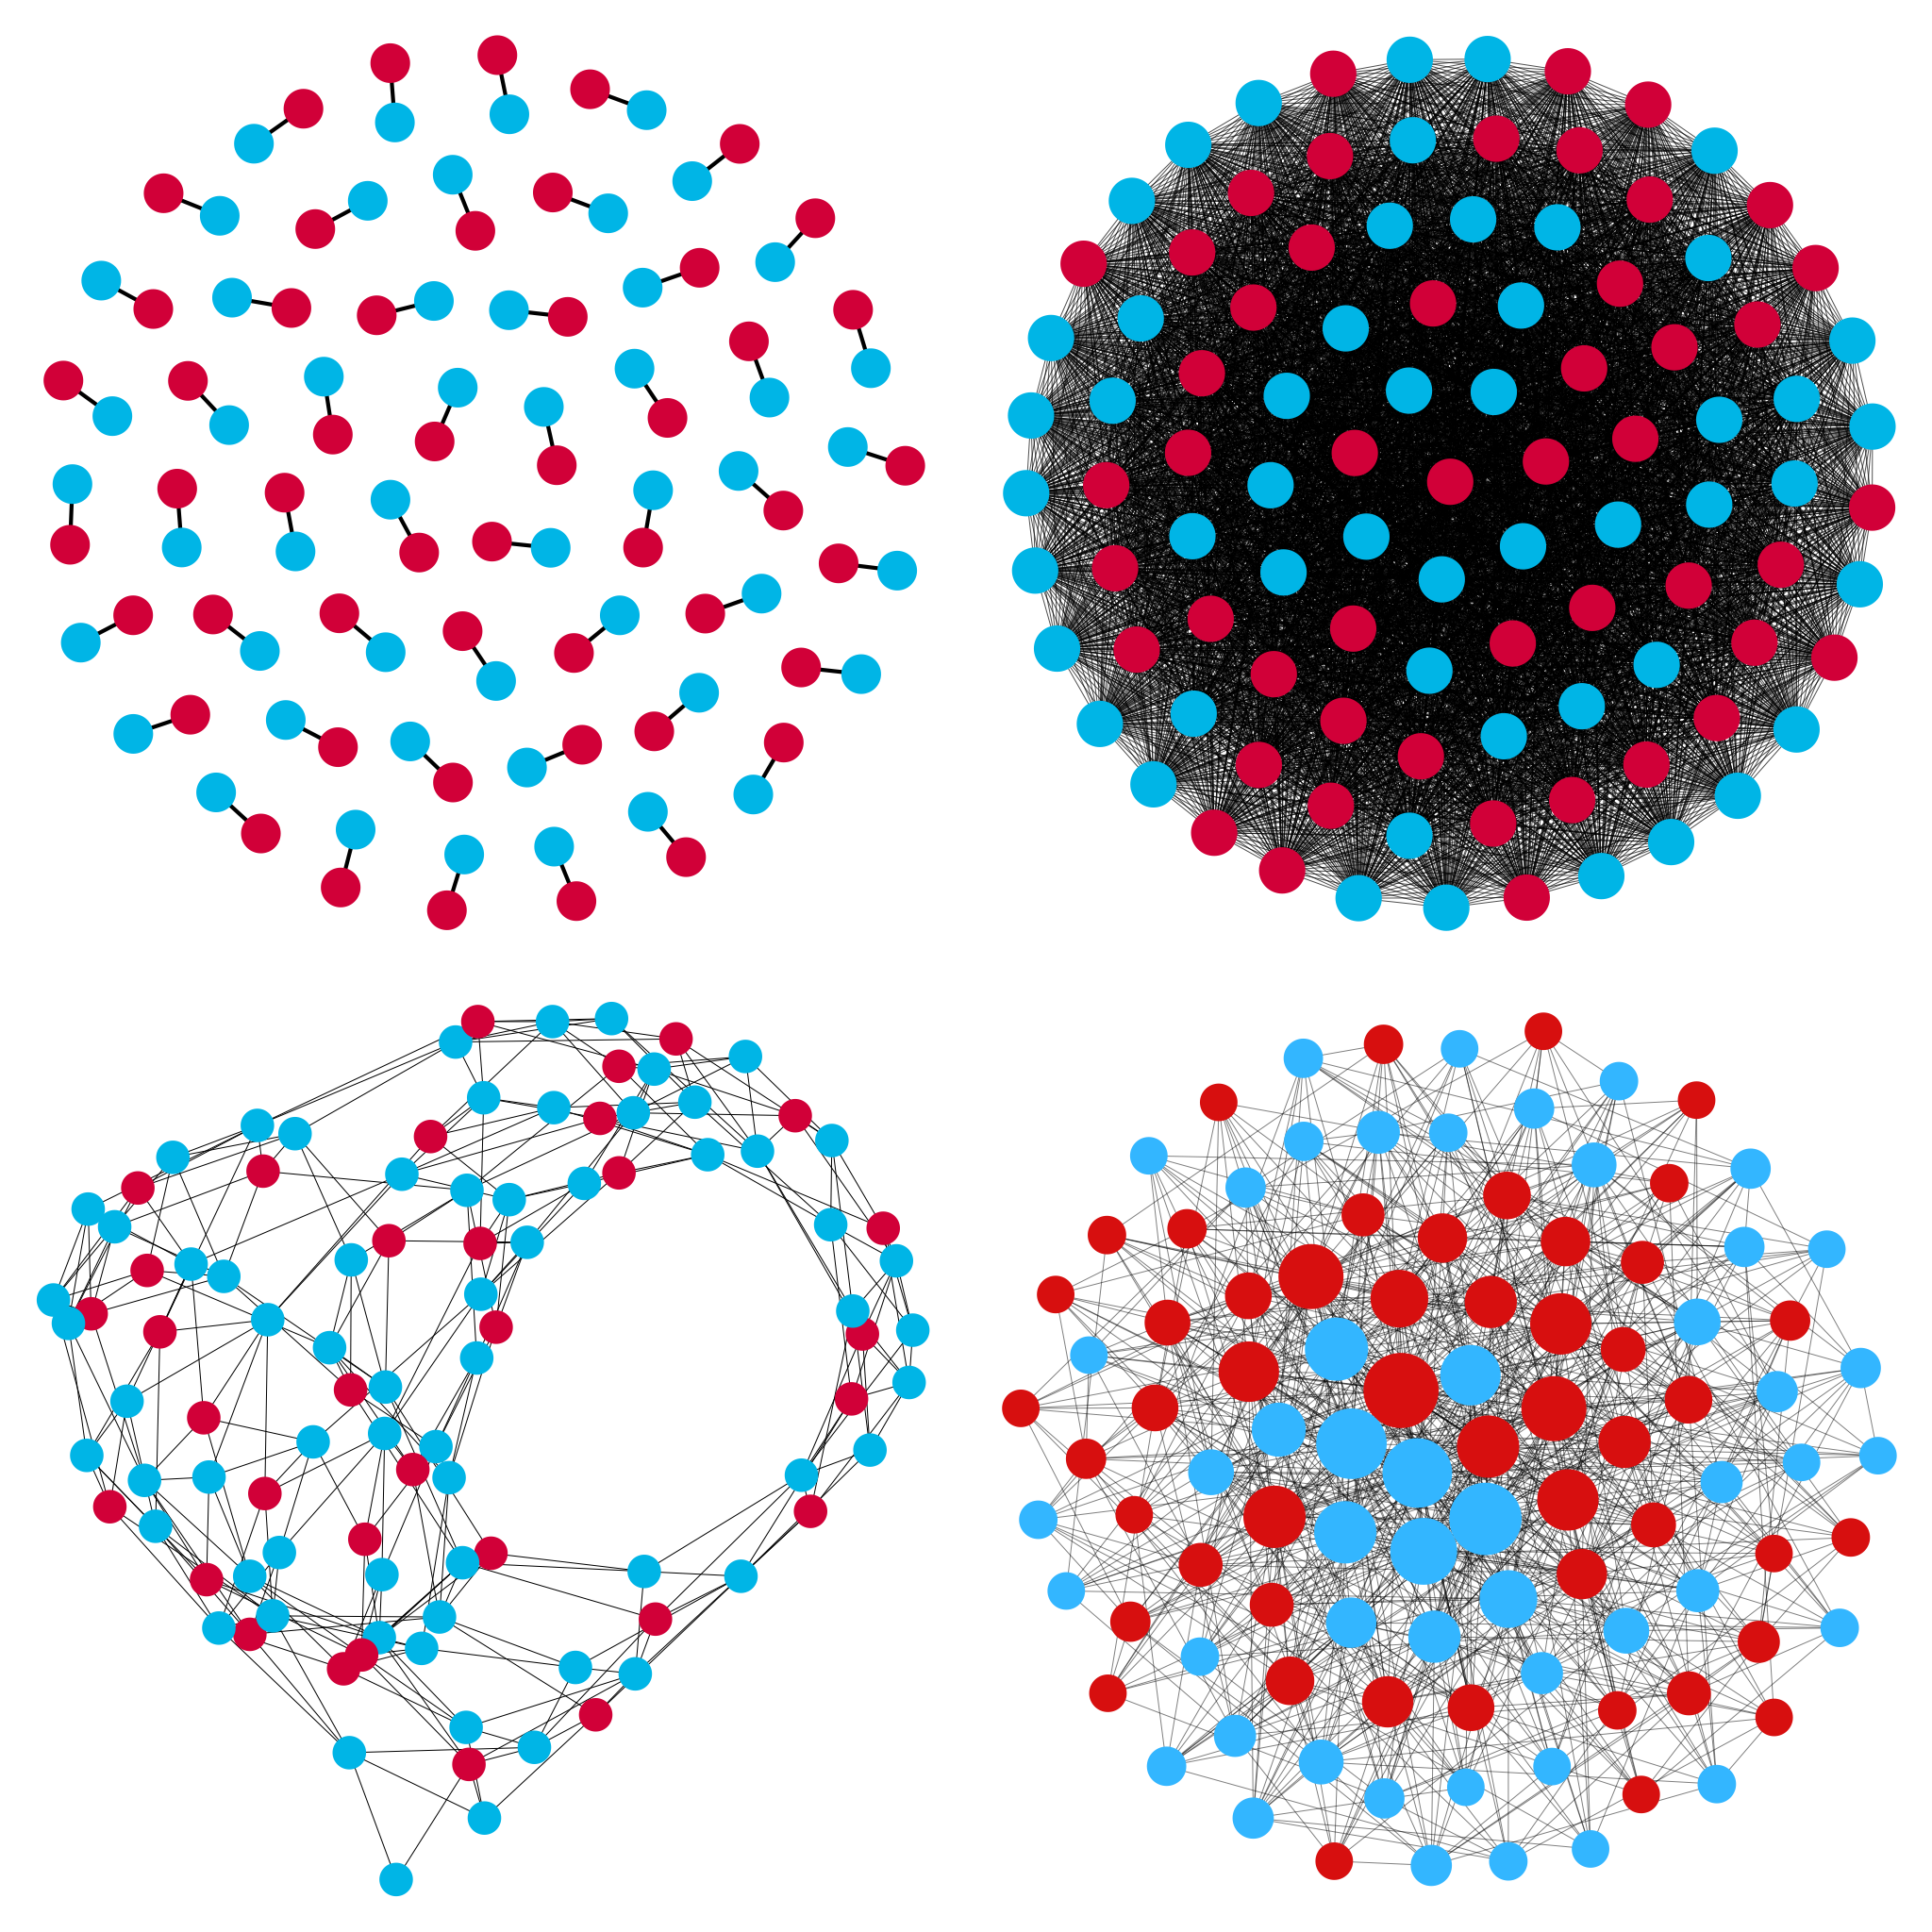
\includegraphics[scale=0.075]{../Images/allSimulations.png}
\end{figure}
\begin{itemize}
\item The institutional mechanisms dictate the resulting structure of the network, the positions of economic agents, and aggregate welfare within the socio-economic space.
\end{itemize}
\end{frame}

\subsection{Entrepreneurship and the entrepreneurial function}

\begin{frame} \frametitle{Chapter 3: Entrepreneurship \& the entrepreneurial function}
\begin{itemize}
\item If the division of labour is at the centre of the relational perspective, then its evolution is of major importance in our discussion.
\medskip
\item We have discussed many of the attributes the socio-economic space: 
\begin{itemize}
\medskip
\item \textbf{The fundamental elements:} Consumer-producers, governance system, and interaction infrastructures; and 
\medskip
\item \textbf{The fundamental forces:} Guidance, networking and embeddedness.
\end{itemize}
\medskip
\item We have still yet to talk about the final force: entrepreneurship and the entrepreneurial function.
\medskip
\item Its definition and illustration is the purpose of this Chapter.
\end{itemize}
\end{frame}


\begin{frame}
\begin{itemize}
\item Consider a socio-economic space with a population of economic agents and a governance system of institutions.
\begin{itemize}
\medskip
\item An \textbf{entrepreneur} is an economic agent who, through her actions, engages in entrepreneurship.
\medskip
\item \textbf{Entrepreneurship} refers to actions that modify in a major way elements of the governance system and the underlying interaction infrastructure in the socio-economic space, thus directly or indirectly impacting the population of the socio-economic space.
\medskip
\item The \textbf{entrepreneurial function} refers to actions that modify in a minor way elements of the socio-economic space, thus directly impacting the individual economic agent and her local environment.
\end{itemize}
\medskip
\item Entrepreneurship is considered as a ``higher form'' of adaptive specialisation, leading to new roles that become embedded and thus subject to objective specialisation.
\end{itemize}
\end{frame}


\begin{frame}
\begin{itemize}
\item This definition of entrepreneurship is related to established theoretical perspectives, but does not fit traditional models of `ocupational choice'.
\begin{itemize}
\medskip
\item Schumpeter (1912, 1935, 1942): New product and process innovations faciliate the emergence of new specialisations and roles.
\medskip
\item Baumol (1990): Entrepreneurship can be either `productive`, `unproductive` or `destructive`. Depends on institutional environment.
\medskip
\item Henrekson and Sanandaji (2011): Entrepreneurs can abide by, evade or alter institutions.
\medskip
\item Burt (1992, 2004, 2010): Entrepreneurs possess and exploit superior social capital through the leveraging of information.
\end{itemize}
\end{itemize}
\end{frame}


\begin{frame}
\begin{itemize}
\item Given the definition of the entrepreneur and the simulations in the previous Chapter we make the following conjecture:
\begin{itemize}
\medskip
\item Through a process of entrepreneurship an economic agent creates a new socio-economic role.
\medskip
\item This role carries unique positional attributes within the interaction infrastructure it exist within.
\end{itemize}
\medskip
\item This conjecture is central to subsequent formal analysis regarding the relationship between entrepreneurship and the interaction infrastructure of the socio-economic space.
\end{itemize}
\end{frame}

\section{Entrepreneurship in a Platonian Economy}

\begin{frame}
\frametitle{Table of contents}
\tableofcontents[currentsection]
\end{frame}

\subsection{Overview of Part II}

\begin{frame} \frametitle{Part II overview}
\begin{itemize}
\item Part I developed the relational perspective and noted the impact the entrepreneurs have on the institutional environment. Part II analyses the relationship between entrepreneurs, network position, and power.
\medskip
\item This Part results in:
\begin{itemize}
\medskip
\item[1.] A set of tools in which to measure entrepreneurial power in networks. This is based on the agents unique position and the connectivity of their environment.
\medskip
\item[2.] A game theoretic model in which to understand entrepreneurship as a coalitional act.
\medskip
\item[3.] Application of these tools to empirical examples; in particular the elite Florentine marriage and exchange network.
\end{itemize}
\medskip
\item This is expressed over two chapters.
\end{itemize}
\end{frame}

\subsection{Middlemen as entrepreneurs}

\begin{frame} \frametitle{Chapter 4: Middlemen as entrepreneurs}
\begin{itemize}
\item Entrepreneurial agents possess unique positions within an interaction infrastructure.
\medskip
\item Centrality tools have been developed to look at nodes that are in ``the thick of things'' (Freeman, 1977). These concentrate on the links that nodes have in the network, the eigenvector of the network, the geodesic paths that they exist on, etc.
\medskip
\item These tools do not highlight the unique positions of entrepreneurial agents. We develop a set of measures that to measure the power of a agent through:
\begin{itemize}
\medskip
\item[a.] The inability for other agents to \emph{contest} the entrepreneurs position;
\medskip
\item[b.] The walks that the entrepreneurial agent can \emph{exploit}; and
\medskip
\item[c.] The \emph{robustness} of their unique position.
\end{itemize}
\end{itemize}
\end{frame}


\begin{frame}
\begin{itemize}
\item All analysis is generalised to directed graphs and therefore the tools developed have no specific application to economic scenarios \emph{per se}.
\medskip
\item Can be used in sociology or information theory to investigate the transfer of knowledge or flow and potential manipulation of information.
\medskip
\item We apply these measures of power and robustness to the marriage network of elite Florentine families and to Krackhardt's managerial advice network.
\medskip
\item The rise of the Medici can be attributed to their unique position in their social network; in particular, their ability to broker relationships between opposing factions in Florence.
\medskip
\item However, their position is not robust relative to other powerful elite families, such as the Pazzi.
\end{itemize}
\end{frame}


\begin{frame}
\begin{figure}[h]
\centering
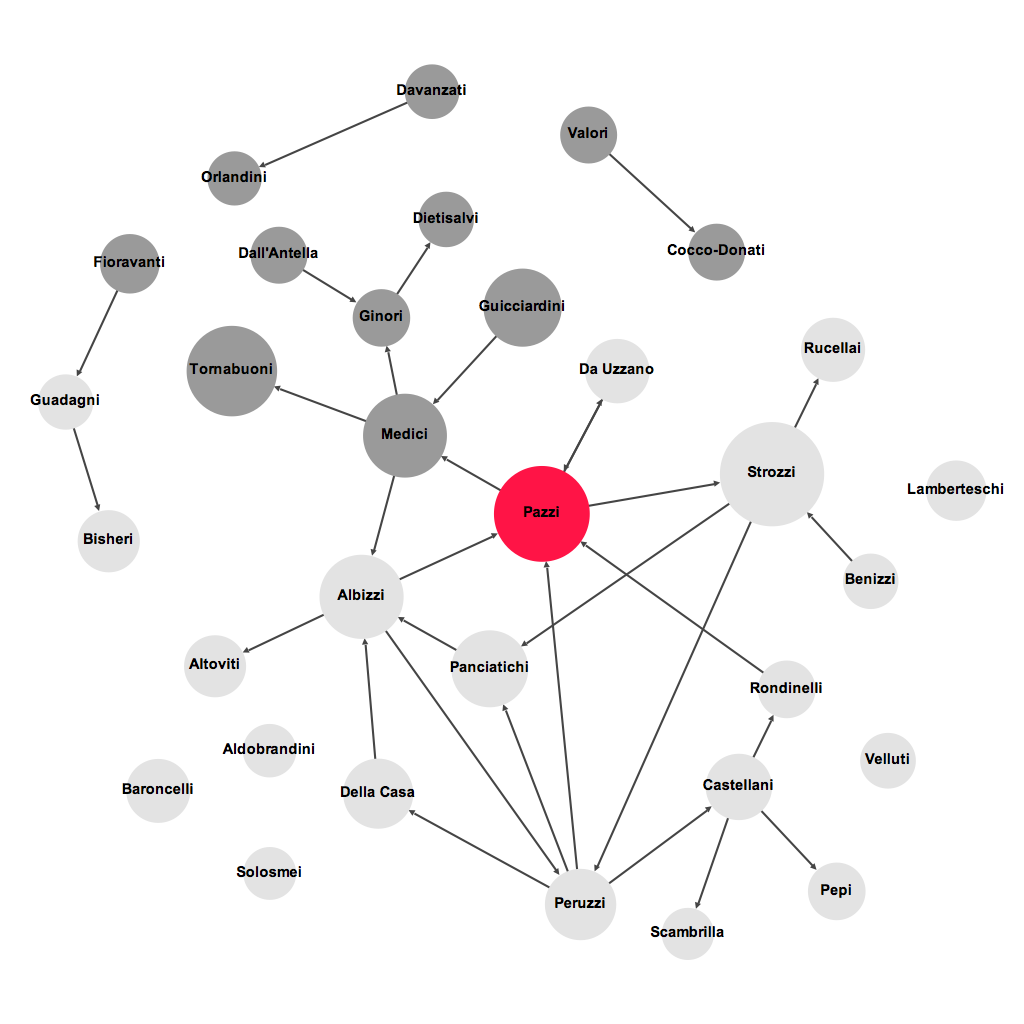
\includegraphics[scale=0.17]{../Images/Florentine-marr.png}
\end{figure}
\begin{itemize}
\item With the tools developed we highlight the powerful brokerage opportunities, which the Medici took advantage of.
\end{itemize}
\end{frame}

\subsection{The formation of extractive structures in networks}

\begin{frame} \frametitle{Chapter 5: The formation of extractive structures in networks}
\begin{itemize}
\item The tools developed in the previous chapter relate to the positional power of individual entrepreneurial agents. It does not consider the network as a structure that can evolve out of strategic decision-making.
\medskip
\item The insights in the previous chapter are generalised to consider coalitions of agents that can attain entrepreneurial power within a given network structure.
\medskip
\item Agents can effectively manipulate the interaction infrastructure in a major way in an effort to reduce their contestability and/or increase their robustness.
\medskip
\item We use game theory in conjunction with graph theory to provide a measurement of entrepreneurial power from group activity.
\end{itemize}
\end{frame}


\begin{frame}
\begin{itemize}
\item Again, we apply these measures to empirical examples of two evolving networks:
\begin{itemize}
\medskip
\item[1.] The marriage network of elite Florentine families; and
\medskip
\item[2.] The network of 9/11 terrorists from 1999--2001.
\end{itemize}
\medskip
\item \textbf{Appendix:} The algorithmic solution to the `blocking problem' discussed in this Chapter is applied to problems of vaccination and network decompartmentalisation.
\end{itemize}
\end{frame}

\section{Entrepreneurship in a Platform Economy}

\begin{frame}
\frametitle{Table of contents}
\tableofcontents[currentsection]
\end{frame}

\subsection{Overview of Part III}

\begin{frame} \frametitle{Part III overview}
\begin{itemize}
\item Part III considers entrepreneurship and power more complex interaction infrastructures. This infrastructure illustrates a vertical division of labour and is represented in terms of a hypergraph: a generalisation of a network.
\medskip
\item This Part results in:
\begin{itemize}
\medskip
\item[1.] Tools that provide an analysis of power and influence of individuals and affiliations within a hypergraph setting.
\medskip
\item[2.] An analysis of the corporate directorate of New York City during the early Twentieth Century.
\medskip
\item[3.] Investigate into the relationship between the topological structure of the economy and the institutional environment.
\end{itemize}
\medskip
\item This is expressed over two chapters.
\end{itemize}
\end{frame}

\subsection{Measuring control in hyperhraphs}

\begin{frame} \frametitle{Chapter 6: Measuring control in hyperhraphs}
\begin{figure}[h]
\centering
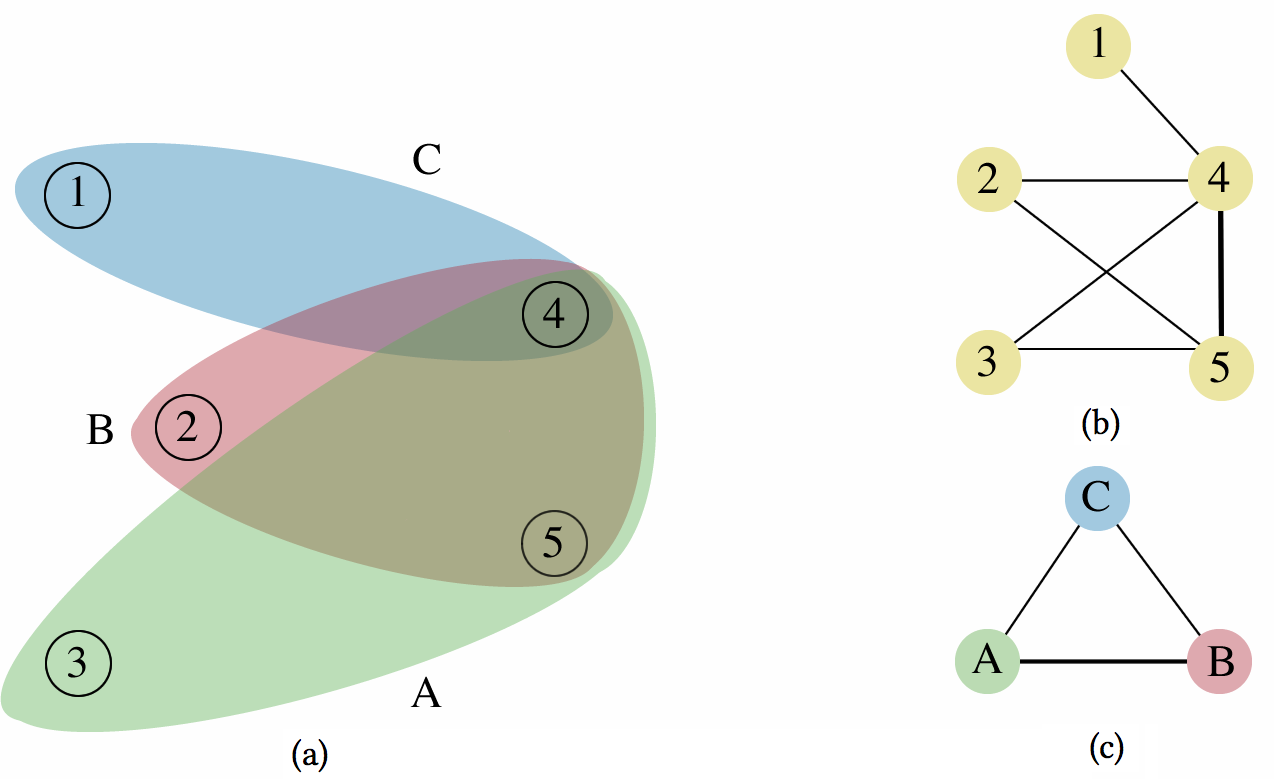
\includegraphics[scale=0.14]{../Images/hypergraph.png}
\end{figure}
\begin{itemize}
\medskip
\item We consider the \textbf{influence} that individual agents and affiliations have in a weighted hypergraph.
\end{itemize}
\end{frame}

\begin{frame}
\begin{itemize}
\item The measurement of influence is derived from the $\beta$-measure (van den Brink and Gilles, 2000) and we prove that it is, in fact, a generalisation of the standard degree measure for networks.
\medskip
\item We also allow affiliations of a hypergraph to be allocated to different \textbf{aspects}; which relate to groups of socio-economic roles.
\medskip
\item A population of \textbf{elites} are derived from the aspectual nature of hypergraphs. These are agents that exist in all aspects of the hypergraph.
\medskip
\item Particular application is applied to indicating important agents in directorate networks.
\end{itemize}
\end{frame}

\subsection{Control in the Platform economy: The case of New York City}

\begin{frame} \frametitle{Chapter 7: Control in the Platform economy: The case of New York City}
\begin{figure}[h]
\centering
\includegraphics[scale=0.15]{../Images/institutions.png}
\end{figure}
\begin{itemize}
\medskip
\item We consider the influence of individuals and firms in the directorate network of NYC.
\end{itemize}
\end{frame}


\begin{frame}
\begin{figure}[h]
\centering
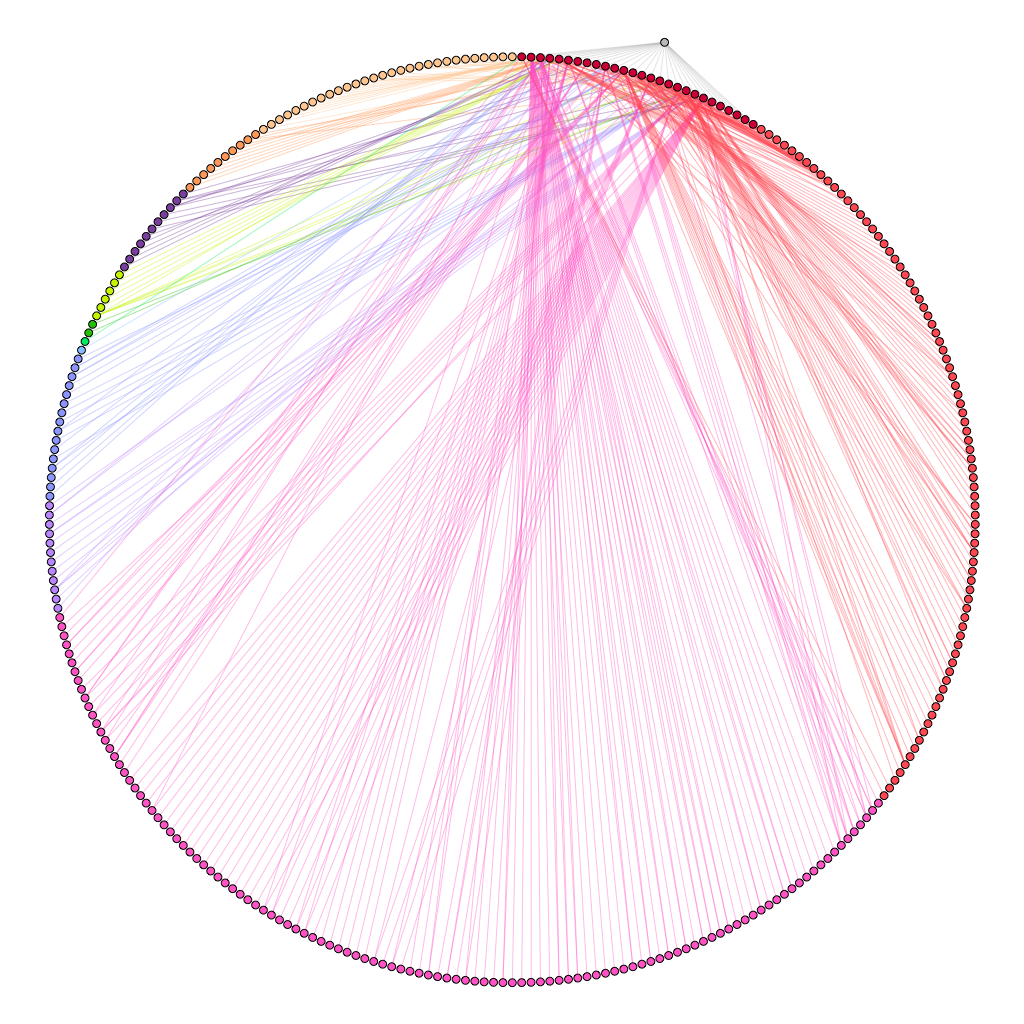
\includegraphics[scale=0.18]{../Images/guarantryBipartite.png}
\end{figure}
\begin{itemize}
\medskip
\item We consider the influence that individual agents and affiliations have in a weighted hypergraph.
\end{itemize}
\end{frame}

\end{document}